\appendix

\section{Hyperparameter Sensitivity}
\label{app:sensitivity}

\begin{table}[t]
\centering
\caption{Clamping (trust region) ablation: success rate (\%) by task with $c_{\max}=0.01$\,m vs.\ vanilla. $n=20$ episodes per cell. \textbf{Caveat:} per-cell $n{=}20$ is small; the pooled row averages across tasks with very different base rates ($35\%$--$90\%$) and is \emph{directional only} --- it carries no claim of statistical significance. We report this ablation as a sensitivity probe, not as a hypothesis test.}
\label{tab:clamping_ablation}
\begin{tabular}{lcc}
\toprule
Task & Vanilla (\%) & Clamp=0.01m (\%) \\
\midrule
Task 4 & 35 & 40 \\
Task 6 & 90 & 90 \\
Task 7 & 30 & 25 \\
Task 8 & 90 & 75 \\
\midrule
Pooled & 61.2 & 57.5 \\
\bottomrule
\end{tabular}
\end{table}

\begin{table}[t]
\centering
\small
\caption{Gating threshold sensitivity ($n=5$ episodes per cell). Success rate (\%) by task and gating configuration.}
\label{tab:gating_ablation}
\begin{tabular}{lcccccccc}
\toprule
Task & Van. & m0.005m & m0.010m & m0.020m & m0.050m & p0.50 & p0.85 & p0.95 \\
\midrule
T4 & 20 & 20 & 20 & 0 & 40 & 40 & 60 & 40 \\
T6 & 100 & 60 & 100 & 80 & 80 & 100 & 80 & 100 \\
T7 & 20 & 20 & 0 & 0 & 0 & 0 & 0 & 0 \\
T8 & 80 & 40 & 40 & 40 & 40 & 40 & 40 & 20 \\
\bottomrule
\end{tabular}
\end{table}


Moderate clamping ($c_{\max}{=}0.01$\,m) preserves base-policy success on easy tasks (Table~\ref{tab:clamping_ablation}). Moderate gating thresholds perform best ($n{=}5$ per cell; Table~\ref{tab:gating_ablation}).

\section{Statistical Details}
\label{app:stats}

\begin{table}[t]
\centering
\caption{Statistical tests on paper-curated pooled LIBERO results. Holm-adjusted $p$-values apply to the three z-tests as one family.}
\label{tab:stat_tests}
\begin{tabular}{lccc}
\toprule
Comparison & $\Delta$ Success (pp) & 95\% CI (pp) & $p$ (z) / Holm \\
\midrule
Steering vs MPPI & -0.38 & [-1.76, +1.00] & 0.5907 / 1 \\
Steering vs Vanilla & -0.31 & [-1.69, +1.07] & 0.6609 / 1 \\
MPPI vs Vanilla & +0.07 & [-1.31, +1.45] & 0.9211 / 1 \\
Steering vs Latent Jiggle & -1.16 & [-2.56, +0.23] & 0.1026 / 1 \\
MPPI vs Latent Jiggle & -0.78 & [-2.18, +0.61] & 0.2721 / 1 \\
Vanilla vs Latent Jiggle & -0.85 & [-2.25, +0.54] & 0.2314 / 1 \\
\midrule
Latent Stop vs Vanilla & -27.61 & [-30.89, -24.32] & 0 \\
\bottomrule
\end{tabular}
\end{table}

\begin{table}[t]
\centering
\caption{TOST equivalence tests ($\pm$2\,pp margin) on paper-curated pool. Equivalence established if $p_{\mathrm{TOST}} < 0.05$.}
\label{tab:equivalence_tost}
\begin{tabular}{lccc}
\toprule
Comparison & $\Delta$ (pp) & $p_{\mathrm{TOST}}$ & Equivalent? \\
\midrule
Steering vs MPPI & -0.38 & 0.01093 & Yes \\
Steering vs Vanilla & -0.31 & 0.008384 & Yes \\
MPPI vs Vanilla & +0.07 & 0.003149 & Yes \\
\bottomrule
\end{tabular}
\end{table}

\begin{table}[t]
\centering
\caption{Stratified difficulty analysis. Hard tasks: vanilla SR $<$30\%; Easy tasks: vanilla SR $>$70\%. Two-proportion z-test on steering vs.\ vanilla.}
\label{tab:stratified_difficulty}
\begin{tabular}{lcccccc}
\toprule
Stratum & \#Tasks & Vanilla (\%) & Steering (\%) & $\Delta$ (pp) & 95\% CI & $p$ (z) \\
\midrule
Hard (SR$<$30\%) & 4 & 19.2 & 20.0 & +0.8 & [-0.9, +2.5] & 0.371 \\
Easy (SR$>$70\%) & 4 & 84.4 & 83.1 & -1.3 & [-2.9, +0.3] & 0.124 \\
\bottomrule
\end{tabular}
\end{table}


\begin{figure}[h]
    \centering
    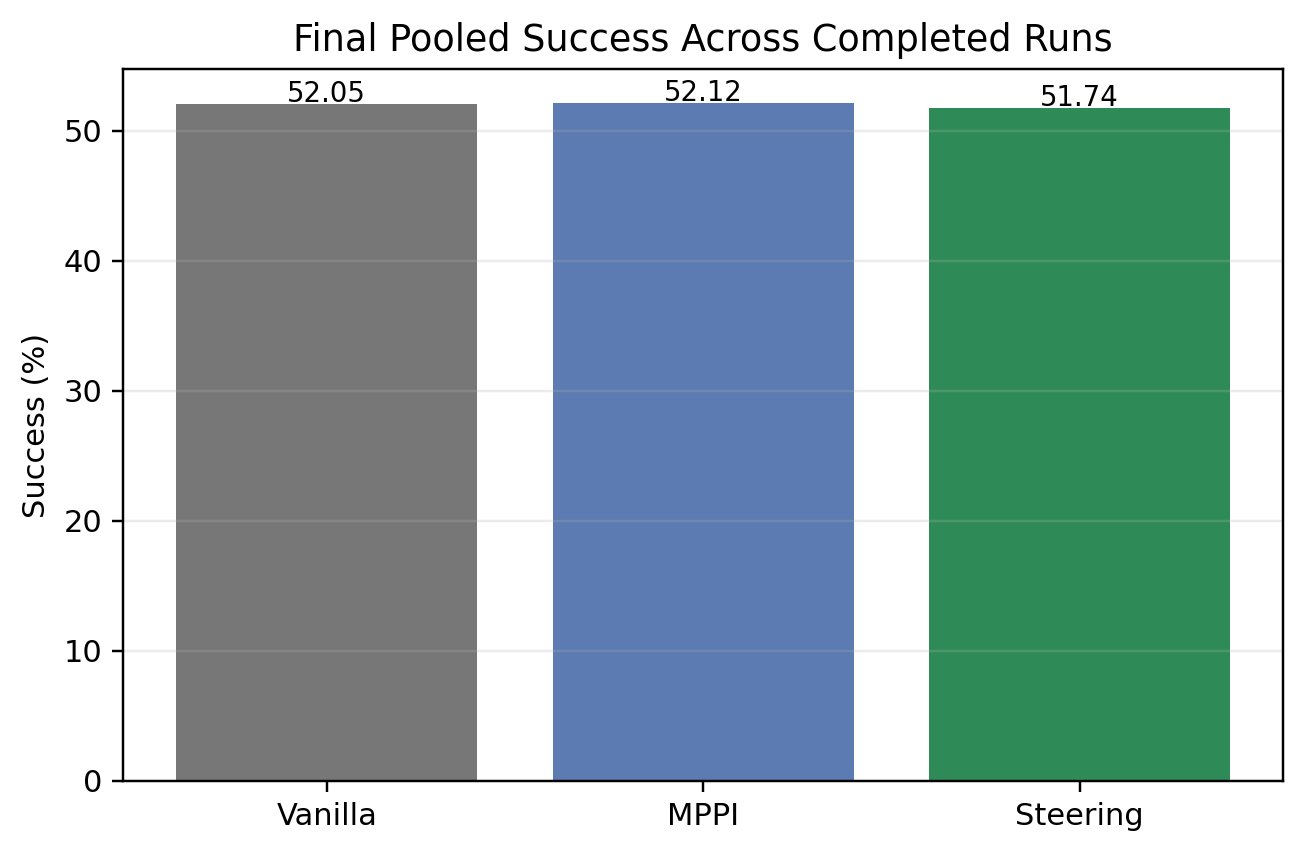
\includegraphics[width=0.7\linewidth]{figures/10_final_pooled_success.png}
    \caption{Pooled success rates across all completed runs.}
\end{figure}

\section{Zero-Shot and OOD Details}
\label{app:zero_shot}

\begin{table}[t]
\centering
\caption{\textbf{ACT strict zero-shot OOD runs} (train-task/test-task splits with disturbance stress). Per-run cells are success rate (\%). \emph{Mean of percentages} averages the six per-run percentages (i.e., treats each run as one observation). \emph{Pooled} sums successes and episodes across all six runs ($n{=}280$ episodes per controller) and is the input to the two-proportion $z$-test in the bottom row. Steering vs.\ Vanilla is statistically indistinguishable in this regime ($+0.71$\,pp pooled, $z{=}0.17$, $p{=}0.86$); Latent Stop is degenerate (zero success because the strict split holds out tasks).}
\label{tab:act_zero_shot_ood}
\resizebox{\linewidth}{!}{%
\begin{tabular}{lccccc}
\toprule
Run & Vanilla & Latent Stop & MPPI & Steering & $\Delta$(Steering$-$Vanilla) \\
\midrule
T0--7 train / T8--9 test, seed s42 & 35.0 & 0.0 & 37.5 & 30.0 & -5.0 \\
T0--7 train / T8--9 test, seed s43 & 25.0 & 0.0 & 35.0 & 35.0 & +10.0 \\
T0--7 train / T8--9 test, seed s44 & 37.5 & 0.0 & 42.5 & 35.0 & -2.5 \\
T2--9 train / T0--1 test, seed s42 & 52.5 & 0.0 & 52.5 & 55.0 & +2.5 \\
T0--5 train / T6--9 test, seed s42 & 40.0 & 0.0 & 37.5 & 38.8 & -1.2 \\
T0--7 train / T8--9 test, stop cfg  & 32.5 & 0.0 & 40.0 & 35.0 & +2.5 \\
\midrule
Mean of run percentages & 37.1 & 0.0 & 40.8 & 38.1 & +1.05 \\
Pooled (successes / $n{=}280$) & 105/280 (37.50) & 0/280 (0.00) & 113/280 (40.36) & 107/280 (38.21) & +0.71 \\
\multicolumn{6}{l}{\quad Steering vs.\ Vanilla pooled: $z{=}0.17$, $p{=}0.862$ (two-proportion); Wilson 95\% CIs $[32.7,44.0]$ vs.\ $[32.0,43.3]$.} \\
\bottomrule
\end{tabular}%
}
\end{table}

\begin{table}[t]
\centering
\caption{\textbf{ACT OOD baseline campaign on hard tasks} (completed seeds, NVIDIA A100). ``MPPI'' is K-sample MPPI search over the PULSE failure head; ``Steering'' is single-step gating on the same head (see \S\ref{sec:experimental_setup}). Latency columns are restricted to the OOD-only run set on the two hardest ACT tasks (tasks 8/9 with OOD push) and are \emph{not} the canonical paper headline; see Table~\ref{tab:final_pooled_results} for the pooled measurement that the $6.1\times$ figure traces to. We report these latencies for completeness so readers can verify that the speedup holds qualitatively across slicings of the data even when the absolute ms values shift with sample composition.}
\label{tab:act_ood_baselines}
\resizebox{\linewidth}{!}{%
\begin{tabular}{lcccccc}
\toprule
Run & Vanilla & Latent Stop & MPPI & Steering & MPPI ms & Steering ms \\
\midrule
act\_ood\_baselines\_s42\_t89 & 54.5 & 46.0 & 56.0 & 50.0 & 2.969 & 0.615 \\
act\_ood\_t89\_s43 & 27.5 & 32.5 & 35.0 & 35.0 & 3.915 & 0.676 \\
\midrule
Aggregate (completed) & 41.0 & 39.2 & 45.5 & 42.5 & 3.442 & 0.645 \\
\bottomrule
\end{tabular}%
}
\end{table}


\begin{figure}[h]
    \centering
    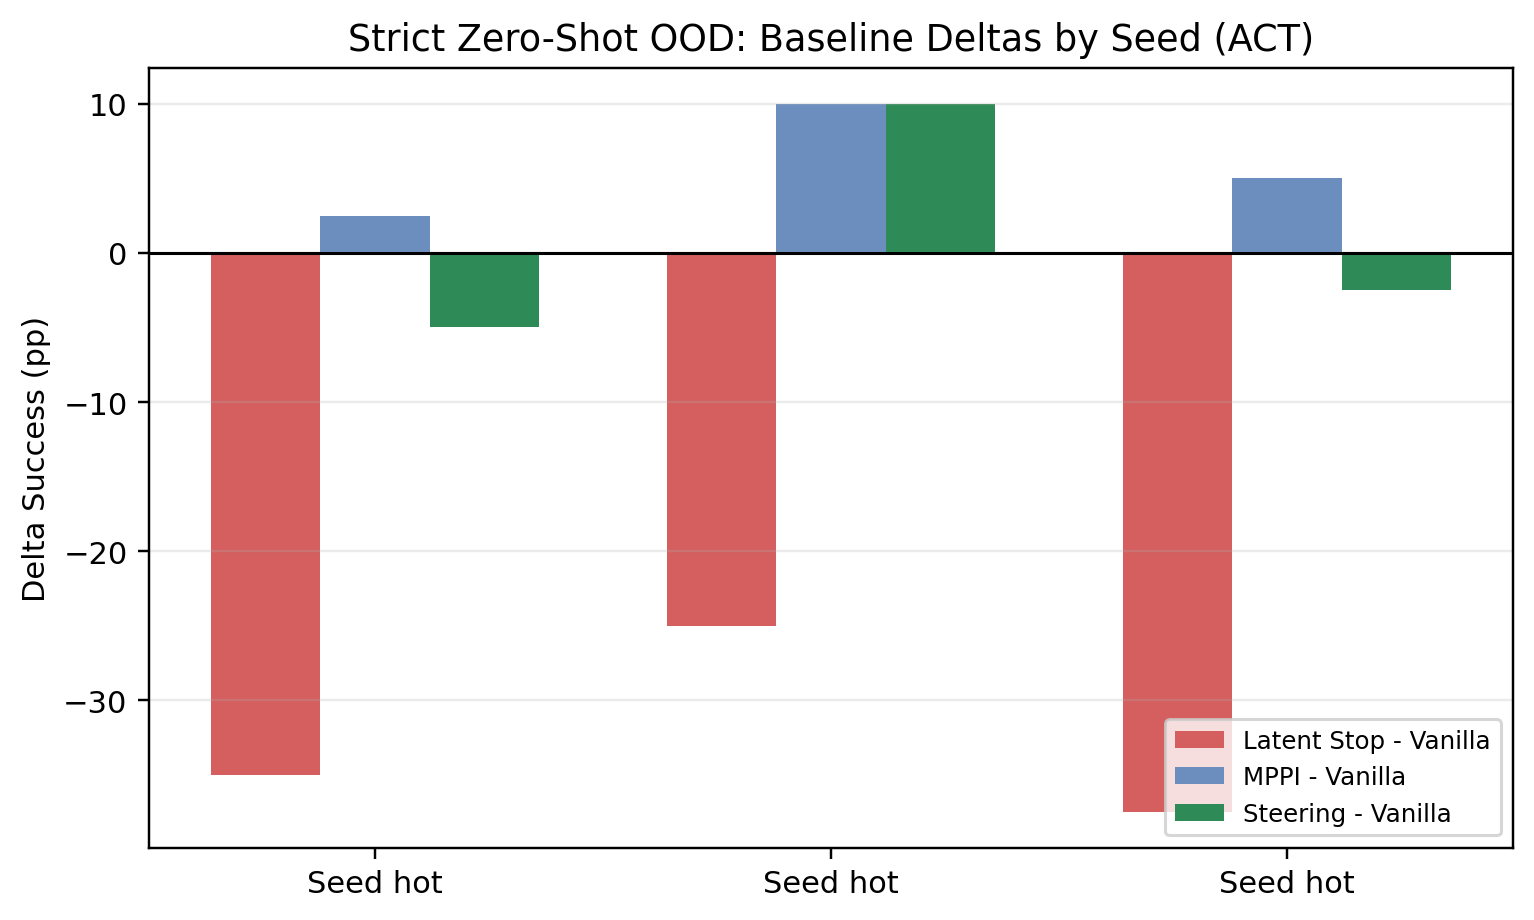
\includegraphics[width=0.8\linewidth]{figures/07_zero_shot_seed_deltas.png}
    \caption{Zero-shot OOD: per-seed deltas vs.\ vanilla.}
\end{figure}

\section{Cross-Model Transfer Details}

\begin{figure}[h]
    \centering
    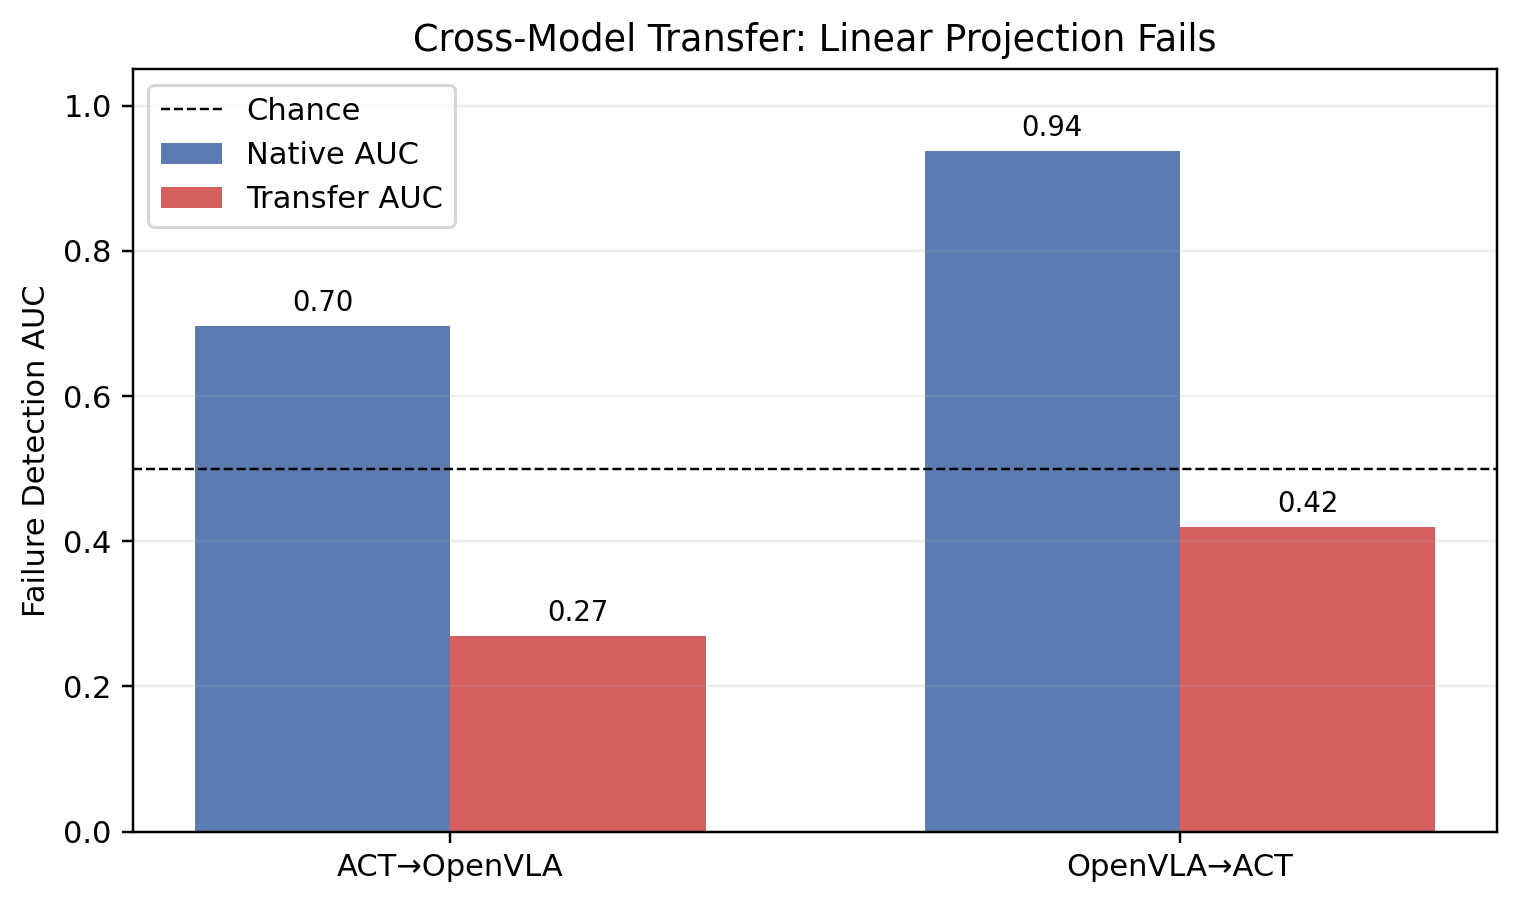
\includegraphics[width=0.65\linewidth]{figures/26_transfer_result.png}
    \caption{Cross-model transfer via linear projection. Native AUCs are strong but transfer drops below chance.}
    \label{fig:transfer}
\end{figure}

\section{OOD Push Sweep Details}

\begin{figure}[h]
    \centering
    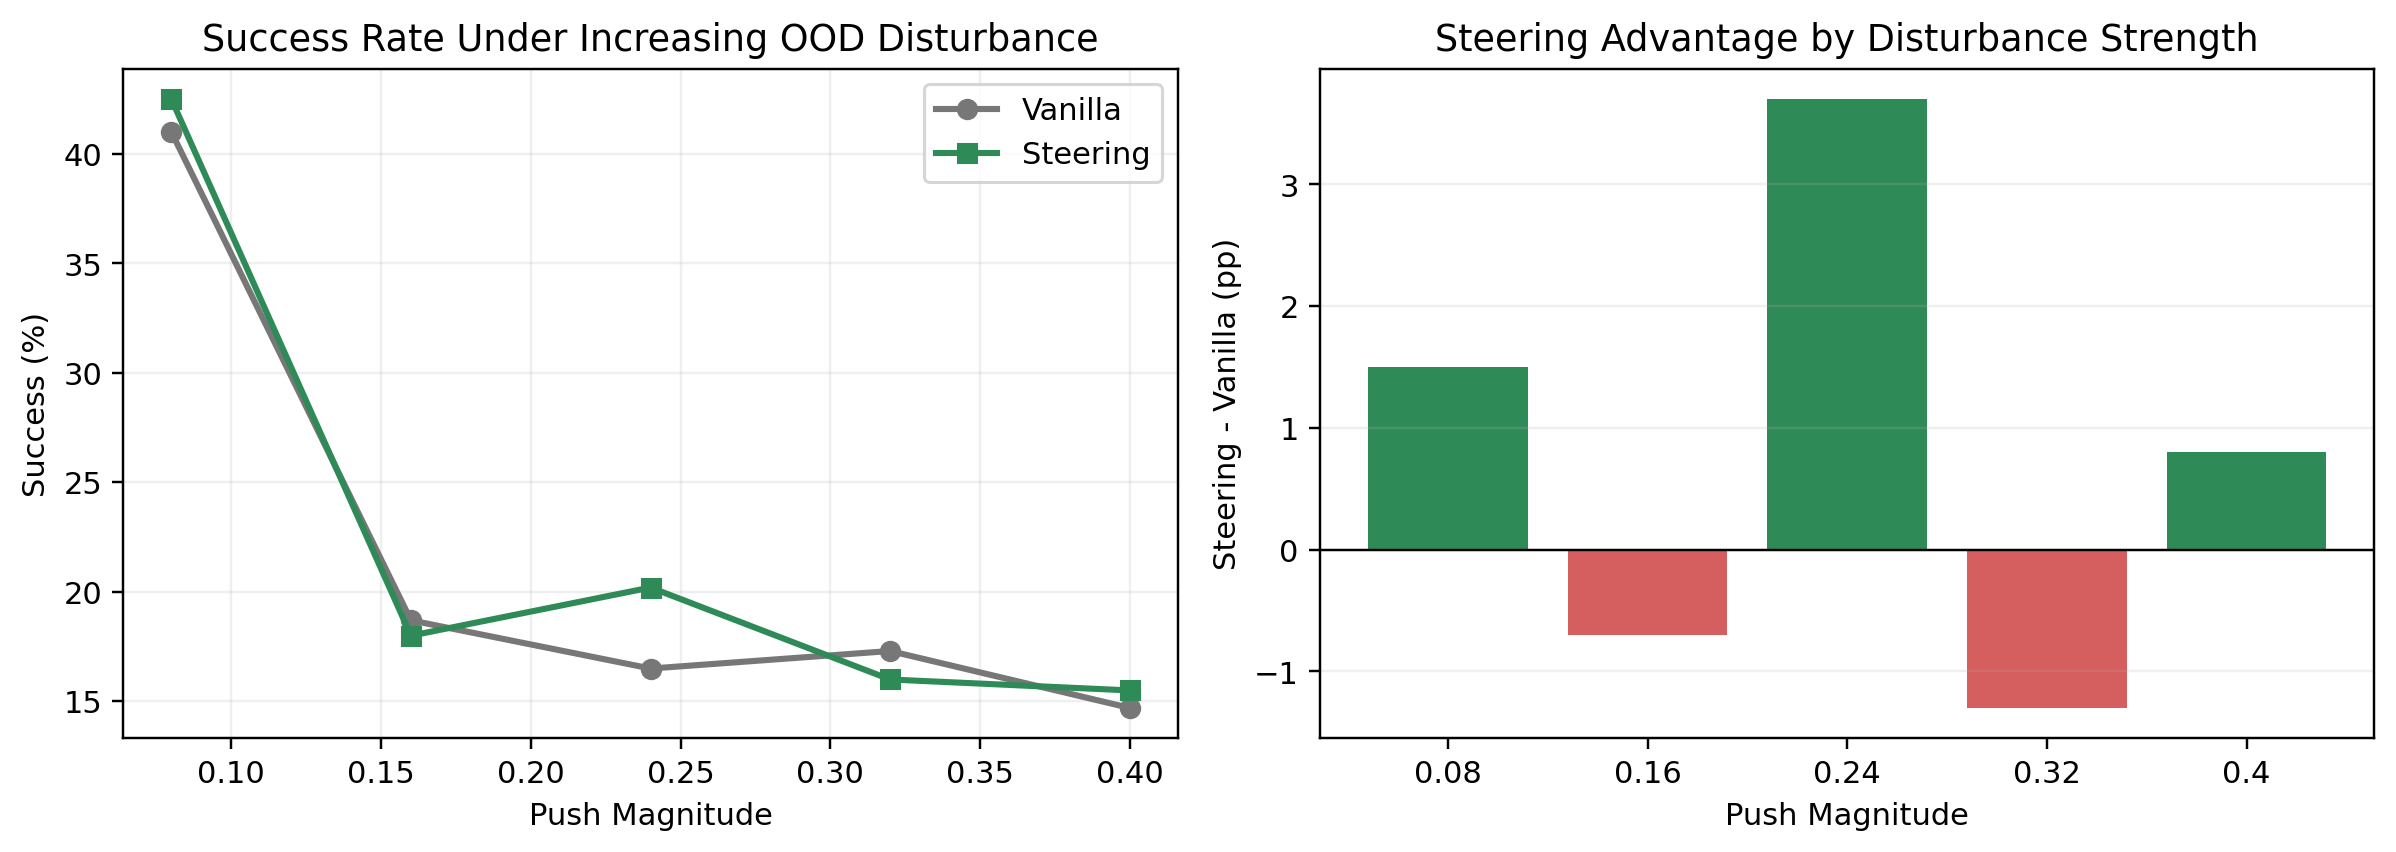
\includegraphics[width=0.78\linewidth]{figures/25_ood_push_sweep.png}
    \caption{Left: success rate under increasing OOD disturbance. Right: steering advantage by push magnitude.}
\end{figure}

\section{Reproducibility}

All metrics map to stored JSON outputs indexed by deterministic run tags. Code, SLURM configs, evaluation pipelines, and safety probe checkpoints for both architectures will be released. Tables regenerate from frozen data via \texttt{run\_stat\_tests.py} and \texttt{generate\_tables.py}.
